\section{Pre Main Sequence}\label{sec:pre-main-sequence}

La fase di pre-MS (pre main sequence) è quella in cui si va a formare una stella, partendo dalla contrazione di una nube di gas. Per far si che questa si formi, però, è necessario che siano presenti determinate condizioni: sia $m$ la massa di una particella di ai margini della nube gassosa (possibilmente una molecola di $H_2$) e si indichi con $R$ la distanza di questa dal centro. Al fine di osservare la formazione di una stella è necessario che l'attrazione gravitazionale agente sulla particella, dal resto della nube, sia maggiore rispetto alla pressione esercitata dal gas su di essa, imponiamo quindi l'equazione~\ref{eq:1}.
\begin{equation}
    G \frac{M m}{R} \geq k_B T
    \label{eq:1}
\end{equation}
Dove $M$ è la massa della nube, $T$ è la temperatura e $k_B$ la costante di Boltzmann.
\subsection{Massa di Jeans}

Considerando che la massa della nube può essere espressa come segue
\[
    M = \frac{4}{3} \pi R^3 \rho
\]
allora possiamo esplicitare la dipendenza del raggio da alcune caratteristiche della nube, in particolare della massa e della densità.
\begin{equation}
    R = \sqrt{\frac{3}{4\pi} \frac{M}{\rho}}
    \label{eq:2}
\end{equation}
Inserendo l'equazione~\ref{eq:2} nella (\ref{eq:1}), si ottiene la relazione come le varie caratteristiche del gas devo essere in modo tale da permettere la formazione di una stella.
\begin{equation}
    M^{\frac{2}{3}} \geq \frac{k_B T}{G m} \sqrt{\frac{3}{4\pi} \frac{1}{\rho}}
    \label{eq:3}
\end{equation}
Sia $a = \sqrt{\frac{3}{4\pi}}\frac{k_B}{G m} \sim \SI{e16}{g.K^{-1}.cm^{-1}}$ una costante, allora si riscrive la relazione~\ref{eq:3} nella forma dell'equazione~\ref{eq:jeans}
\begin{equation}
    M \geq a^{\frac{3}{2}} T^{\frac{3}{2}} \rho^{-\frac{1}{1}}
\label{eq:jeans}
\end{equation}

Questa è la massa necessaria a permettere la contrazione, assumendo che la densità di gas sia uniforma e il valore minimo che soddisfa questa disuguaglianza viene detto massa di Jeans, la quale dipende dai valori di densità e temperatura del gas. In particolare, per temperature elevate e gas rarefatti questa risulta maggiore rispetto al caso con gas densi e relativamente freddi. Di conseguenza si deduce che l'ambiente più favorevole alla formazione stellare è proprio quest'ultimo.

Benché il modello costruito permette di trovare le condizioni iniziali necessarie a favorire la nascita di una stella, il meccanismo che attiva l'effettivo collasso gravitazionale non è ancora ben noto. Le ipotesi più probabili sono quelle dello Shock Front, cioè la compressione dovuta all'esplosione di una supernova, della collisione tra nubi o all'interazione con una galassia.
\subsection{Initial mass function}
Si consideri ora di essere in condizioni interstellari ($T = \SI{10}{K}$ e $ \bar \rho = \SI{e-23}{g.cm^{-2}} $), allora per formare una stella sarebbe necessaria una massa di circa $100 \;M_\odot $, ma noi osserviamo stelle anche decisamente meno massive. Questo significa che in realtà tale meccanismo favorisce la formazione di vari aggregati stellari, con processi frammentati riferiti alla nube iniziale. Definiamo ora con IMF (initial mass function) la distribuzione di massa della stella in formazione all'interno di una popolazione stellare, utile per studiare i passaggi che una data stella attraversa durante la sua evoluzione, in particolare questo valore permette di avere una stima delle seguenti grandezze:
\begin{description}
    \item[Destino] di una stella, cioè quale percorso una stella seguirà nella parte finale della sua vita;
    \item[Durata della vita] di una stella, indica l'ordine di grandezza del tempo necessario alla sua evoluzione;
    \item[Inquinamento] di una stella, ovvero i tipi di elementi chimici che essa rilascia nell'universo nelle ultime fasi della propria vita.
\end{description}

Essendo la IMF una funzione di natura empirica, le sue caratteristiche non sono ancora ben conosciute. Questo significa che non è ben chiaro quale sia la forma di tale funzione e nemmeno se valga in maniera universale, ovvero se sia indipendente dal tempo, caratteristiche della nube o, addirittura, dalla posizione nello spazio. Un'ipotesi del suo andamento vuole che questa prenda la forma dell'equazione~\ref{eq:IMF}.
\begin{equation}
    \Psi(M) = k M^{-s}
    \label{eq:IMF}
\end{equation}
Dove $s$ è un numero positivo e $k$ una costante di proporzionalità.

Si osserva che se il modello dovesse avere questa forma, allora la percentuale di stelle massive è decisamente minore rispetto a quella di stelle con massa relativamente piccola. Tale predizione viene confermata dal fatto che la morte di una stella molto massiva produce un implosione sul nucleo stesso generando una supernova, ma nel nostro cielo tali avvenimenti non sono così comuni. L'andamento della IMF è mostrato nella figura~\ref{fig:IMF}.

\begin{figure}
    \centering
    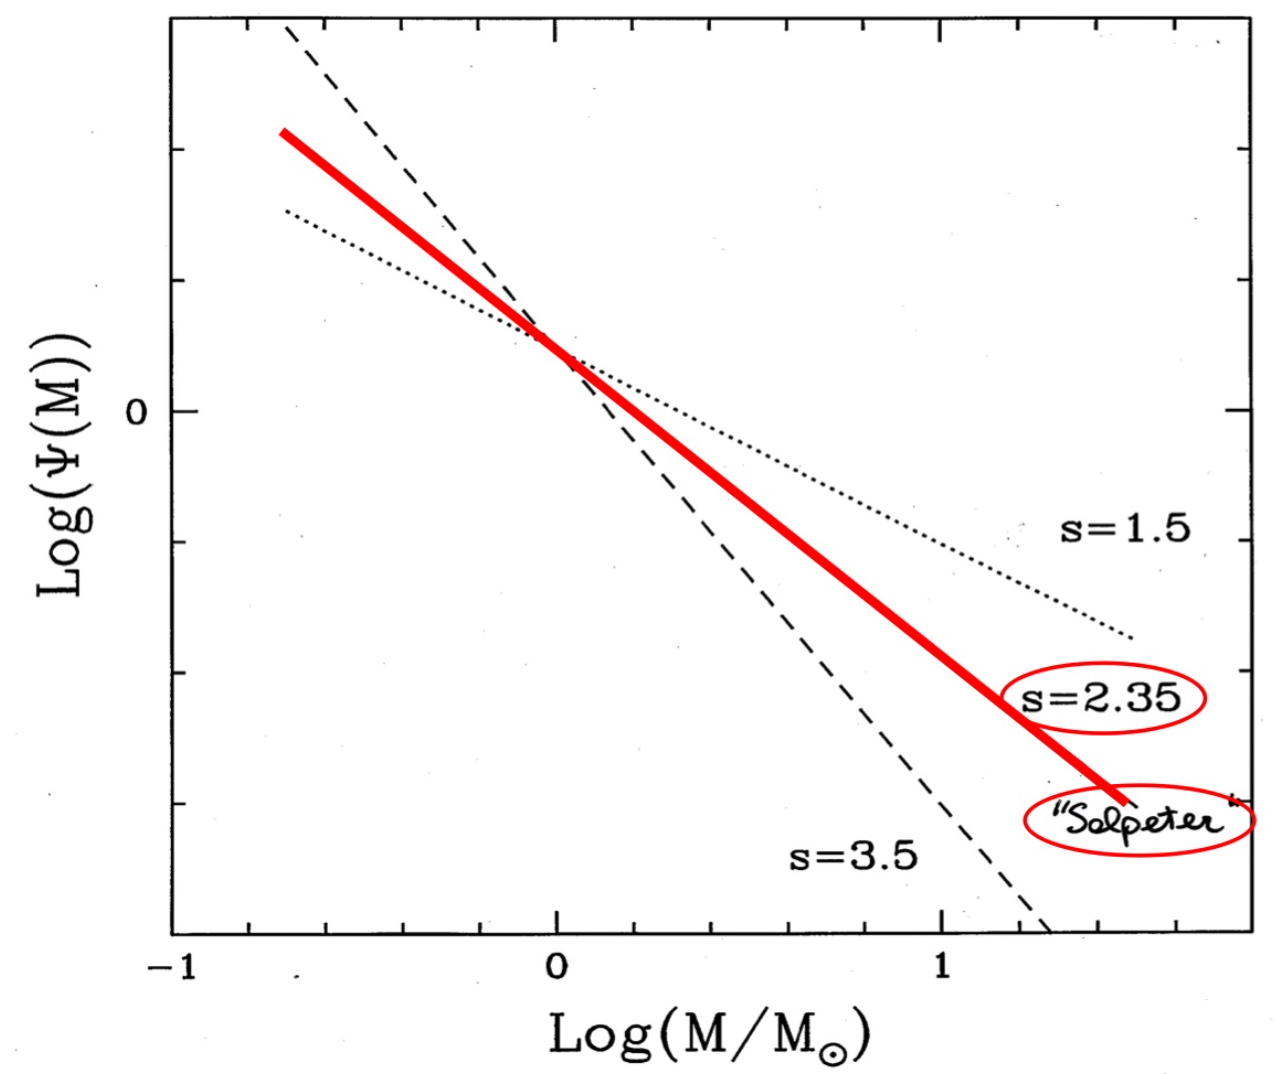
\includegraphics[width = 0.3\textwidth]{immagini/IMF.png}
    \caption{La figura mostra l'andamento della IMF in funzione della massa (normalizzata a quella solare) in scala logaritmica. La presenza di più linee è dovuta al fatto che non è presente una stima unica del parametro $s$ e di conseguenza sono indicate varie possibilità per questo parametro dove in rosso si ha quella più probabile.}\label{fig:IMF}
\end{figure}
\subsection{Protostelle e Teorema di Hayashi}

Data ora una nube di gas non uniforme, questa si inizierà a frammentare verso le varie buche di potenziale gravitazionale, se questi frammenti avranno una massa che soddisfa il criterio di Jeans (\ref{eq:jeans}), allora potrà verrà innescato il collasso gravitazionale, producendo quelle che vengono chiamate Protostelle. Quando la contrazione innesca le reazioni termonucleari, generando un equilibrio idrostatico tra pressione gravitazionale e pressione di radiazione, la stella sarà completamente convettiva. Questo stato può essere rappresentato nel diagramma H-R come un punto della traccia di Hayashi. Si tratta di una linea nel piano H-R che data una stella con una determinata composizione chimica, mostra al variare della massa un punto del diagramma in cui la stella è in equilibrio idrostatico e completamente convettiva. Tale curva quindi mostra una famiglia di stelle con la stessa composizione chimica, ma differente massa iniziale.

Il teorema di Hayashi afferma, inoltre, che fissata la composizione chimica e la massa si una stella, esiste una regione del piano H-R dove non è possibile realizzare modelli stellari in equilibrio idrostatico, la cui traccia di Hayashi funge da bordo. In figura~\ref{fig:hay} è mostrata la zona in questione colorata in rosso, mentre in colorata di verde si ha la regione che permette di avere modelli stabili, parzialmente convettivi. La validità di questo teorema è generale,  continua quindi a valere per ogni punto dell'evoluzione stellare, in modelli convettivi e non.

\begin{figure}
    \centering
    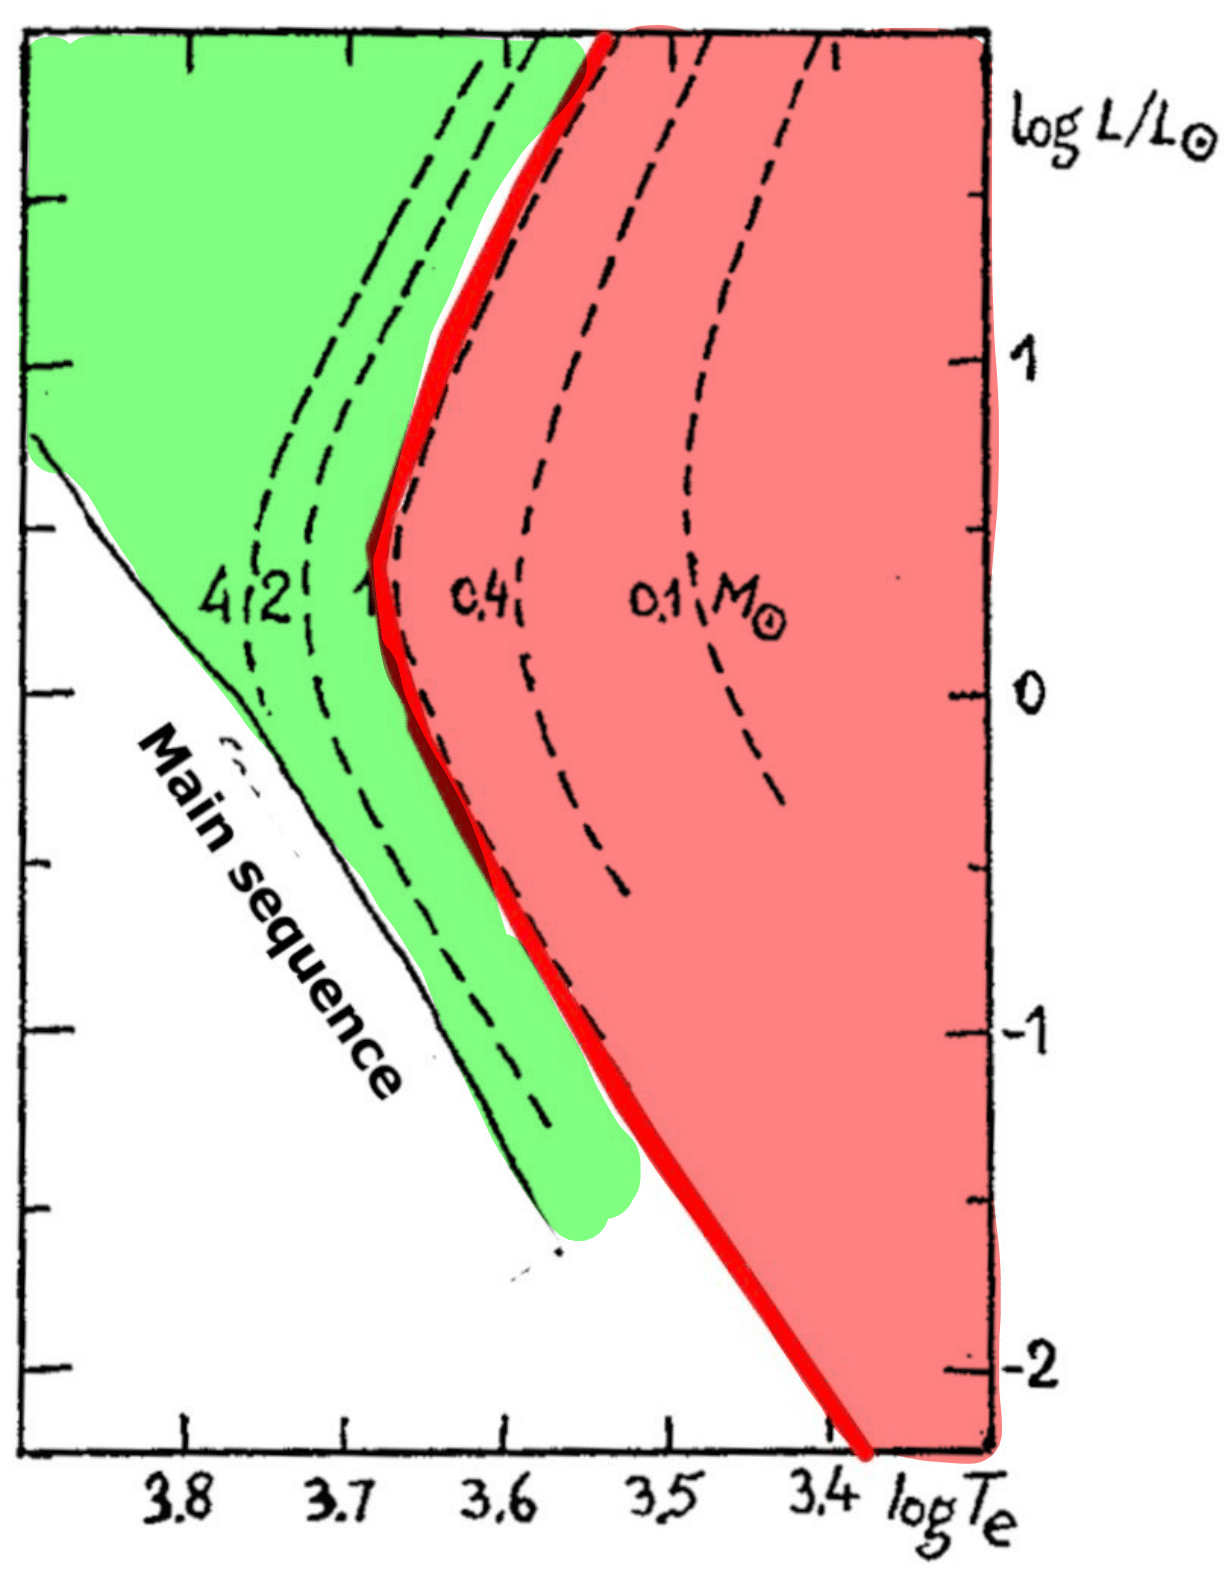
\includegraphics[width = 0.3 \textwidth]{immagini/hayashi-1.png}
    \caption{La figura mostra un diagramma H-R dove è stata evidenziata la traccia di Hayashi in rosso. A destra e a sinistra di questa sono state evidenziate due regioni, una in rosso ed una in verde. La prima mostra la zona in cui non è possibile generare stelle in equilibrio idrostatico, mentre la seconda mostra una regione di stabilità parzialmente convettiva.}\label{fig:hay}
\end{figure}

Particolarmente importante è la posizione di questa zona d'instabilità e della conseguente traccia di Hayashi. Infatti, queste si trovano nella parte fredda del diagramma H-R e, per quanto visto precedentemente, minore la temperatura, maggiore sarà l'opacità della stella. Questo implica un gradiente radiativo maggiore di quello adiabatico ($\nabla_{\mbox{rad}} > \nabla_{\mbox{ad}}$) e quindi la presenza di convezione.

La fase di protostella dura fino a quando il nucleo raggiunge una temperatura $T \sim \SI{e7}{K}$, necessaria ad attivare le reazioni termonucleari. La durata di questa fase della vita della stella è compresa tra i $10^4$ e i $10^7$ anni, a seconda della massa iniziale della stella (maggiore è la massa iniziale, minore sarà la durata). Si tratta di una parte relativamente breve dell'evoluzione stellare.